% !TEX encoding = UTF-8
% !TEX TS-program = pdflatex
% !TEX root = ../tesi.tex

%**************************************************************
\chapter{Verifica e validazione}
\label{cap:verifica_validazione}
%**************************************************************
Ultima fase del periodo di tirocinio è stato svolto dal processo di verifica e validazione. La prima è un processo che si occupa di fornire evidenza oggettiva, ovvero che i risultati ottenuti come output dello sviluppo del software soddisfino i requisiti, la seconda invece è un processo per confermare in modo definitivo che le caratteristiche del software siano conformi ai bisogni dell'utente e all'uso previsto.
Per eseguire la verifica e la validazione è necessario l'esecuzione di test\footnote{In ambito informatico i test eseguiti nel processo di verifica sono eseguiti in maniera automatica durante lo sviluppo del software} che individuino carenze, correttezza e affidabilità. Nel progetto della Skill Concierge Croccante non è stato realizzato alcun test per il processo di verifica: viste le tempisti non è stato ritenuto necessario e si è pertanto scelto di eseguire test già esistenti nel servizio Amazon Lambda, sufficienti ad esaminare il codice e rilevare eventuali errori. Per quanto riguarda il processo di validazione\footnote{Attività di supporto la quale accerta che il prodotto dei processi rispetti le specifiche} è stato svolto, alla fine del periodo di tirocinio, un incontro  con il tutor aziendale e CFO Damiano Buscemi come conferma fiale la quale ha accertato le bontà richieste dal prodotto finale. Tale validazione non è stata altro che una dimostrazione funzionante della Skill, eseguita prima da me per spiegare spiegare le varie funzionalità, ed infine da Crispy Bacon come conferma.
\\[0.5cm]
\noindent Per quanto riguarda l'integrazione coi servizi utilizzati, nello specifico Google Calendar e Slack, sono stati creati dei file appositi da eseguire manualmente che verificano il corretto funzionamento di essi restituendo un risultato:
\begin{figure}[H]
	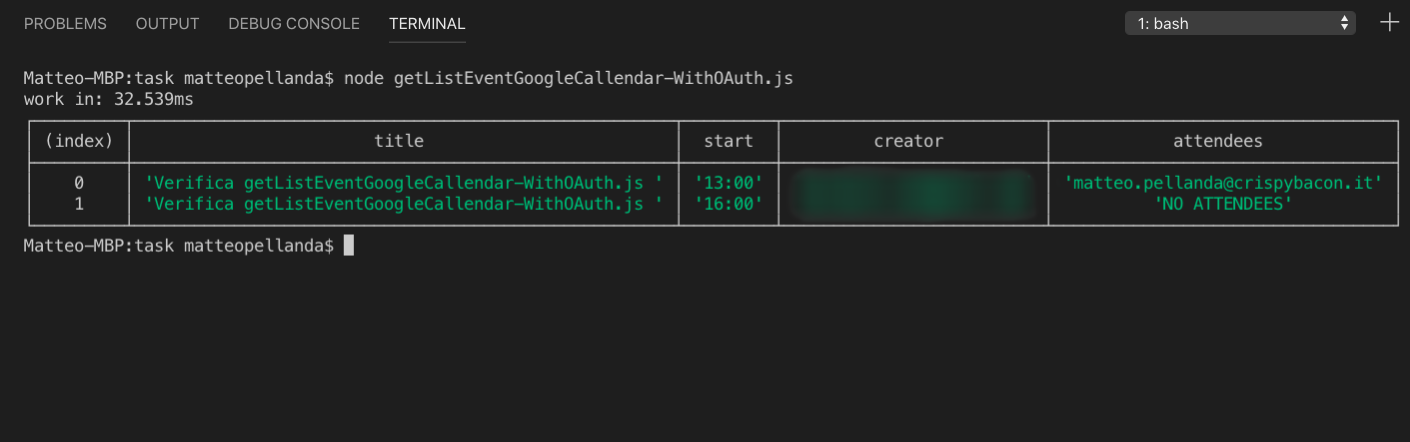
\includegraphics[width=13cm]{immagini/test-googleCalendar.png}
	\caption{\label{fig:test_googleCalendar}Esempio test funzionamento Google Calendar - Lista eventi}
\end{figure}
\newpage
\noindent L'immagine mostra l'esecuzione del file getListEventGoogleCallendar-WithOAuth.js adibito a verificare la validità del token OAuth per ottenere la lista di eventi della giornata corrente. Inoltre verifica la corretta chiamata dell'API \texttt{calendar.events.list}.
\begin{figure}[H]
	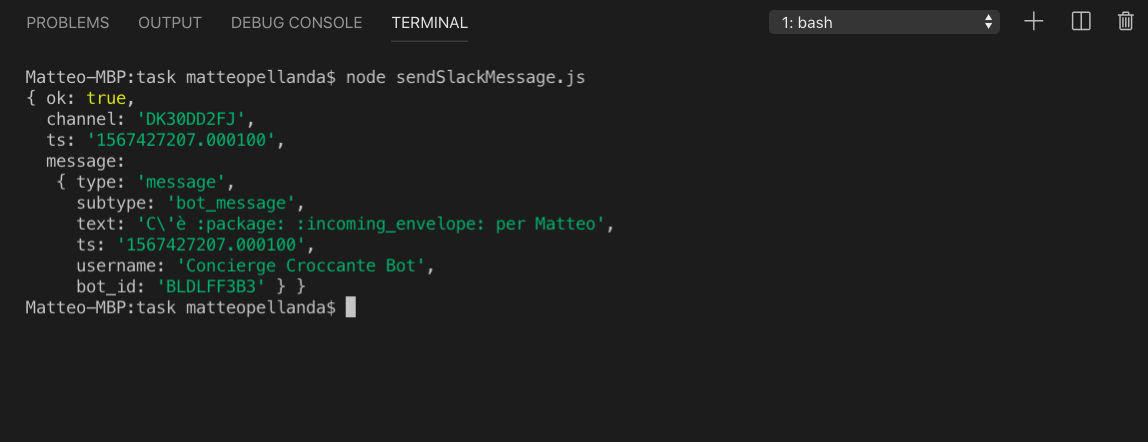
\includegraphics[width=13cm]{immagini/test-sendSlack.png}
	\caption{\label{fig:test_slack_send}Esempio test funzionamento Slack - Invio messaggio}
\end{figure}
\noindent L'immagine mostra l'esecuzione del file sendSlackMessage.js adibito a verificare la validità del token per inviare messaggi di notifica via Slack. Inoltre verifica la corretta chiamata dell'API \texttt{chat.postMessage}.
\begin{figure}[H]
	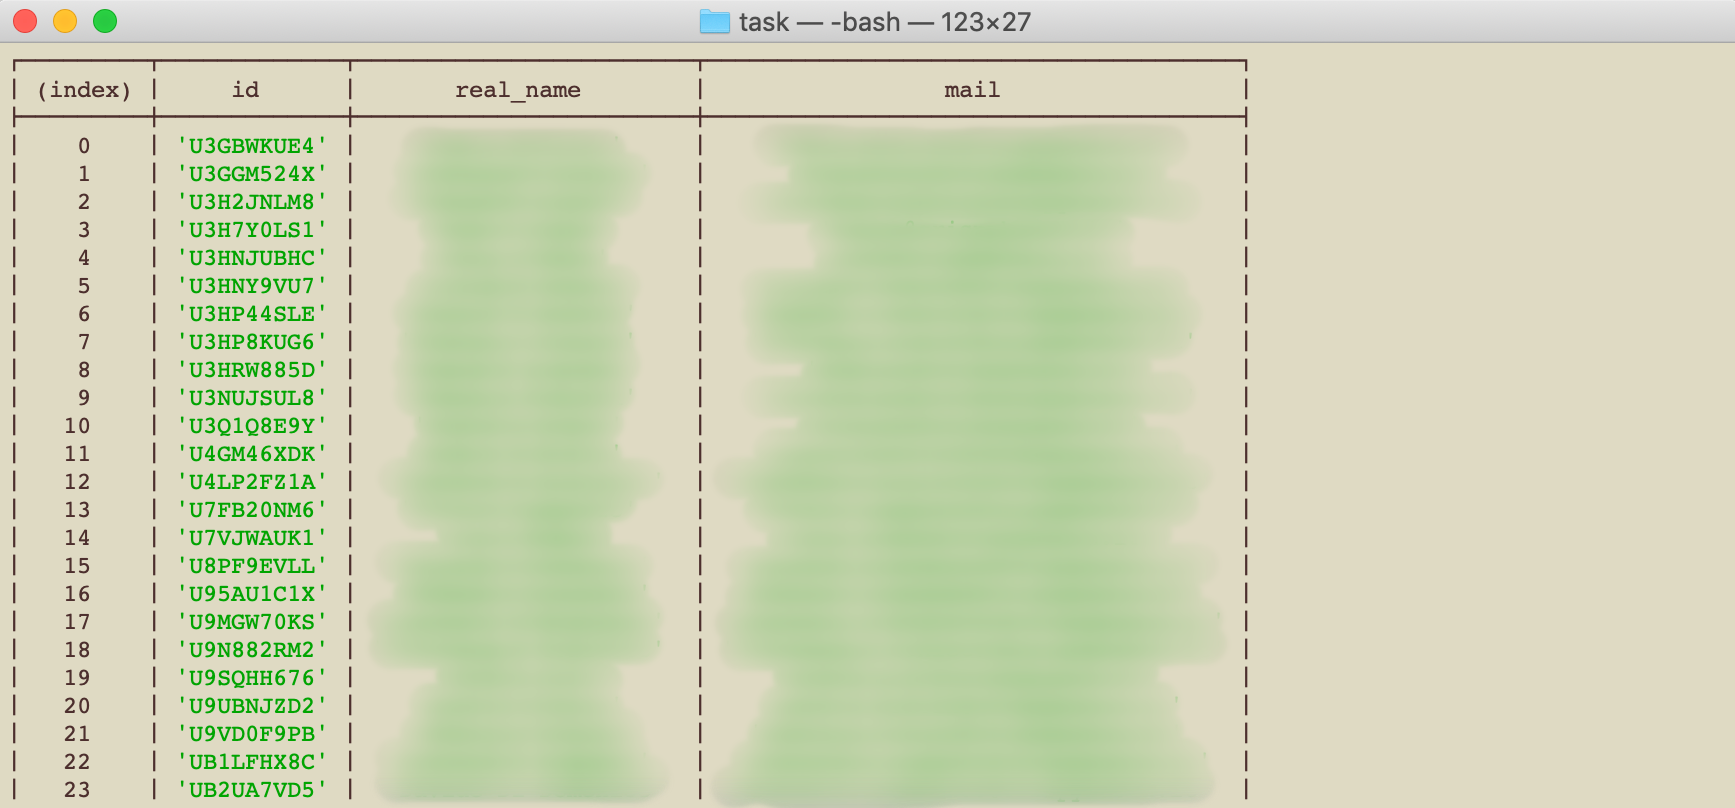
\includegraphics[width=13cm]{immagini/test-listSlack.png}
	\caption{\label{fig:test_slack_list}Esempio test funzionamento Slack - Lista membri}
\end{figure}
\noindent L'immagine mostra l'esecuzione del file getSlackListMemebers.js adibito a verificare la validità del token per ottenere la lista dei membri di Crispy Bacon. Inoltre verifica la corretta chiamata dell'API \texttt{users.list}.
